\documentclass{article}
\usepackage[left=1in,right=1in,top=1in,bottom=1in]{geometry}
\usepackage{amsmath, amsthm, verbatim, enumerate, totcount}
\usepackage[usenames,dvipsnames]{xcolor}
\usepackage{enumerate, tikz, booktabs}
\usepackage{wrapfig}
\usepackage{hyperref}
\usepackage{mathpartir}
\usepackage{listings}
\usepackage{fancyhdr}
\usepackage{pythonhighlight}
\usepackage{graphicx}
\usetikzlibrary{automata,positioning,arrows}


\pagestyle{fancy}
\fancyhf{}
\rhead{My Dinh}
\lhead{CS 458: Introduction to Information Security}
\cfoot{\thepage}

\setlength\parindent{0pt}
\setlength{\parskip}{1em}
\renewcommand{\thesubsection}{\thesection.\arabic{subsection}}

\title{IIT CS458: Introduction to Information Security\\
  {\large Homework 2: Secret-Key Encryption}}
\author{My Dinh}
\date{}

\begin{document}
\maketitle

\addtocounter{section}{1}

\section{Lab Tasks}

\subsection{Task 1: Frequency Analysis}

For the first task, I used Python3 to write a program for cryptanalysis. This
program includes functions for preprocessing text (remove special characters and newline),
counting letter frequency, doubled letter word, one-letter words, two-letter words,
three-letter words, initial letters, final letters.

\begin{python}
import re


# remove special characters and new line
def process_text(text) -> str:
    return re.sub('[^A-Za-z0-9 ]+', '', text.replace("\n", " ")).strip()


# sort the keys in given word dictionary d by their frequency
def sort_frequency(d) -> list:
    return sorted(d, key=lambda x: -d[x])


# count letter frequency in text
def count_letters(text) -> dict:
    d = {}

    for c in text:
        if c.isalpha():
            d.setdefault(c, 0)
            d[c] += 1

    return d


# count words in the text with given length n
def count_words(words, n) -> dict:
    d = {}
    for w in words:
        if len(w) == n:
            d.setdefault(w, 0)
            d[w] += 1
    return d


# count initial letter frequency
def count_initial(words) -> dict:
    d = {}

    for w in words:
        d.setdefault(w[0], 0)
        d[w[0]] += 1

    return d


# count final letter frequency
def count_final(words) -> dict:
    d = {}

    for w in words:
        d.setdefault(w[-1], 0)
        d[w[-1]] += 1

    return d


# count doubled letter frequency
def count_doubled(words) -> dict:
    d = {}

    for w in words:
        for i in range(len(w)-1):
            if w[i] == w[i+1]:
                d.setdefault(w[i], 0)
                d[w[i]] += 1

    return d


if __name__ == "__main__":
    f = open("./ciphertext.txt")

    text = process_text(f.read())
    words = text.split(" ")

    letter_freq = count_letters(text)
    doubled_freq = count_doubled(words)
    one_letter_words = count_words(words, 1)
    two_letter_words = count_words(words, 2)
    three_letter_words = count_words(words, 3)
    initial_freq = count_initial(words)
    final_freq = count_final(words)

    print(letter_freq)
    print(sort_frequency(letter_freq))
    print(sort_frequency(doubled_freq))
    print(sort_frequency(one_letter_words))
    print(sort_frequency(two_letter_words))
    print(sort_frequency(three_letter_words))
    print(sort_frequency(initial_freq))
    print(sort_frequency(final_freq))

    f.close()
\end{python}

Running the program above would give the following result

\begin{center}
    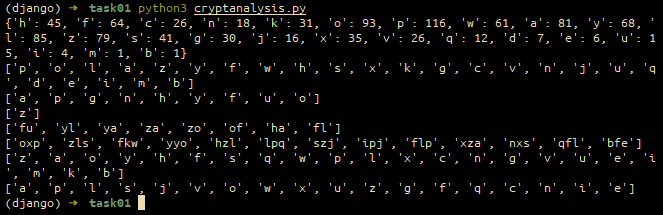
\includegraphics[scale=0.68]{task01.png}
\end{center}

Since the plaintext of the encrypted message is in English, the Cryptanalysis
Form from Class Activity 1 can be used again to analyze the ciphertext.

\begin{enumerate}
    \item
        \begin{itemize}
            \item Most frequent English letters: \textbf{e t a o i n s}
            \item Ciphertext frequencies
                \begin{figure}[!h]
                    \makebox[1 \textwidth][c]{
                        \begin{tabular}{| c | c | c | c | c | c | c | c | c | c | c | c | c | c | c | c | c | c | c | c | c | c | c | c | c | c |}
                            \hline
                            A & B & C & D & E & F & G & H & I & J & K & L & M & N & O & P & Q & R & S & T & U & V & W & X & Y & Z \\
                            \hline
                            81 & 1 & 26 & 7 & 6 & 64 & 30 & 46 & 4 & 16 & 31 & 85 & 1 & 18 & 93 & 116 & 12 & 0 & 41 & 0 & 15 & 26 & 61 & 35 & 68 & 79 \\
                            \hline
                        \end{tabular}
                    }
                \end{figure}
        \end{itemize}
    \item
        \begin{itemize}
            \item 1-letter English words: \textbf{a i}
            \item One letter word in ciphertext: \textbf{z}
        \end{itemize}
    \item
        \begin{itemize}
            \item Most frequently doubled letters in English: \textbf{s e t f l m o}
            \item Double letters in ciphertext: \textbf{a, p, g, f, y, h, n, u}
        \end{itemize}
    \item
        \begin{itemize}
            \item Most frequent 2-letter words in English: \textbf{an, at, as, he, be, in, is, it, on, or, to, of, do, go, no, so, my}
            \item Two-letter words in ciphertext: \textbf{fu, yl, ya, za, zo, of, ha, fl}
        \end{itemize}
    \item
        \begin{itemize}
            \item Most frequent 3-letter words in English: \textbf{the, and, for, was, his, not, but, you, are, her}
            \item Three-letter words in ciphertext: \textbf{oxp, zls, fkw, yyo, hzl, lpq, szj, ipj, flp, xza, nxs, qfl, bfe}
        \end{itemize}
    \item
        \begin{itemize}
            \item Most frequent initial letters in English: \textbf{t a s o i}
            \item Initial letters in ciphertext: \textbf{z, a, o, y, h, f, s, q, w, p, l, x, c, n, g, v, u, e, i, m, k, b}
        \end{itemize}
    \item
        \begin{itemize}
            \item Most frequent final letters in English: \textbf{e s d n t}
            \item Final letters in ciphertext: \textbf{a, p, l, s, j, v, o, w, x, u, z, g, f, q, c, n, i, e}
        \end{itemize}
\end{enumerate}

Using \texttt{tr} tool to map the letters in the ciphertext back to the plaintext,
the result is

\begin{center}
    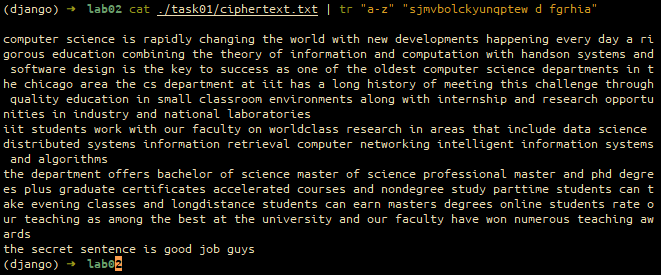
\includegraphics[scale=0.68]{task01_2.png}
\end{center}

The original message is

\textbf{computer science is rapidly changing the world with new developments happening
every day a rigorous education combining the theory of information and computation
with handson systems and software design is the key to success as one of the oldest
computer science departments in the chicago area the cs department at iit has a
long history of meeting this challenge through quality education in small classroom
environments along with internship and research opportunities in industry and national
laboratories}

\textbf{iit students work with our faculty on worldclass research in areas that include
data science distributed systems information retrieval computer networking
intelligent information systems and algorithms}

\textbf{the department offers bachelor of science master of science professional master
and phd degrees plus graduate certificates accelerated courses and nondegree
study parttime students can take evening classes and longdistance students can
earn masters degrees online students rate our teaching as among the best at the
university and our faculty have won numerous teaching awards}

\textbf{the secret sentence is good job guys}

\subsection{Task 2: Encryption using Different Ciphers and Modes}

The ciphertext in \texttt{plain.txt} is \texttt{"A Leetcode a day keeps the unemployment
away."}.

\begin{figure}[!ht]
    \centering
    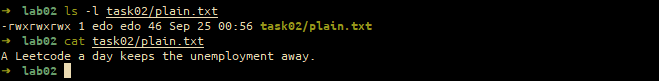
\includegraphics[scale=0.68]{task02_plain.png}
    \caption{Task 2 plaintext information.}
\end{figure}

For this task, I am going to use cipher types \texttt{des}, \texttt{aes-128},
and \texttt{aes-256} with mode types \texttt{ecb}, \texttt{cbc}, and \texttt{cfb}.

\subsubsection{DES}

The \textbf{key} used in this encryption is \texttt{0001020304050607}.

The \textbf{initial vector} used in this encryption is \texttt{0a0b0c0d0e0f0102}
(the initial vector is not needed in ECB mode).

The following figures (\textit{Figure 2, 3, 4}) are the reported results of using
encryption type \texttt{DES} with mode \texttt{ECB}, \texttt{CBC}, and \texttt{CFB}.
The results give us the information about the ciphertext binary and the size of
ciphertext.

\begin{figure}[!ht]
    \centering
    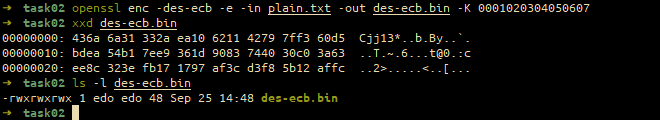
\includegraphics[scale=0.68]{task02_1.png}
    \caption{Cipher type DES with mode ECB.}
\end{figure}

\begin{figure}[!ht]
    \centering
    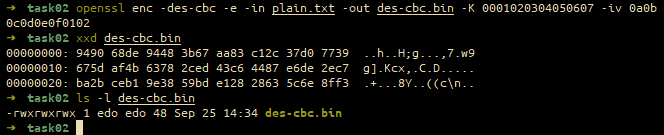
\includegraphics[scale=0.68]{task02_2.png}
    \caption{Cipher type DES with mode CBC.}
\end{figure}

\begin{figure}[!ht]
    \centering
    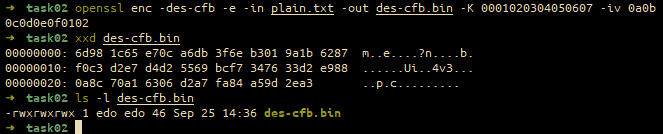
\includegraphics[scale=0.68]{task02_3.png}
    \caption{Cipher type DES with mode CFB.}
\end{figure}

\subsubsection{AES-128}

The \textbf{key} used in this encryption is \texttt{00010203040506070809aabbccddeeff}.

The \textbf{initial vector} used in this encryption is \texttt{0a0b0c0d0e0f010203040506070809}
(the initial vector is not needed in ECB mode).

The following figures (\textit{Figure 5, 6, 7, 8, 9}) are the reported results of using
encryption type \texttt{AES-128} with mode \texttt{ECB}, \texttt{CBC}, and \texttt{CFB}.
The results give us the information about the ciphertext binary and the size of
ciphertext.

\begin{figure}[!ht]
    \centering
    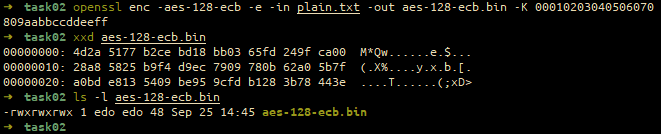
\includegraphics[scale=0.68]{task02_4.png}
    \caption{Cipher type AES-128 with mode ECB.}
\end{figure}

\begin{figure}[!ht]
    \centering
    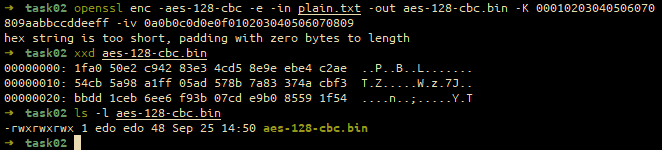
\includegraphics[scale=0.68]{task02_5.png}
    \caption{Cipher type AES-128 with mode CBC. (1)}
\end{figure}

(I understood that I should have chosen a better initial vector to match with the
size of plaintext but I was too lazy and \texttt{openssl} was smart enough to
let me do that by doing padding to the initial vector)

I tried again with a larger size initial vector \texttt{0a0b0c0d0e0f00010203040506070809}
and it stopped printing out the error.

\begin{figure}[!ht]
    \centering
    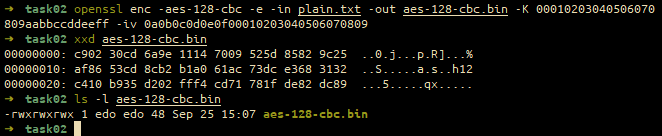
\includegraphics[scale=0.68]{task02_6.png}
    \caption{Cipher type AES-128 with mode CBC. (2)}
\end{figure}

Notice that by changing the position of the zero bytes from the end of the
middle initial vector (in the first case with smaller initial vector, zero bytes
will be added at the end) to the middle of initial vector, the ciphertext would
look completely different.

\begin{figure}[!ht]
    \centering
    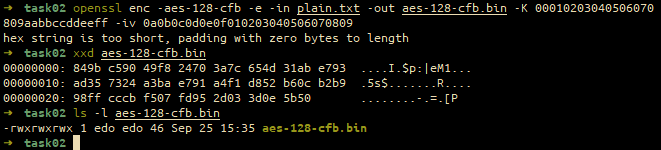
\includegraphics[scale=0.68]{task02_9.png}
    \caption{Cipher type AES-128 with mode CFB. (1)}
\end{figure}

\begin{figure}[!ht]
    \centering
    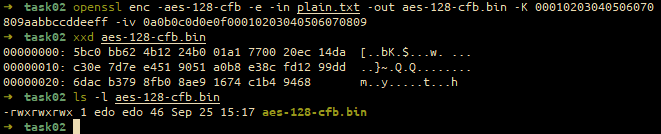
\includegraphics[scale=0.68]{task02_7.png}
    \caption{Cipher type AES-128 with mode CFB. (2)}
\end{figure}

\subsubsection{AES-256}

The \textbf{key} used in this encryption is \texttt{00010203040506070809aabbccddeeff}.

Notice that the size of the key in the lab writeup (or the one given above) is
much smaller than the requirement size of \texttt{aes-256} key (which is 256 bits).
\texttt{openssl} will fix that by performing padding to add zero bytes at the
end of the key.

The \textbf{initial vector} used in this encryption is \texttt{0a0b0c0d0e0f00010203040506070809}
(the initial vector is not needed in ECB mode).

The following figures (\textit{Figure 10, 11, 12}) are the reported results of using
encryption type \texttt{AES-256} with mode \texttt{ECB}, \texttt{CBC}, and \texttt{CFB}.
The results give us the information about the ciphertext binary and the size of
ciphertext.

\begin{figure}[!ht]
    \centering
    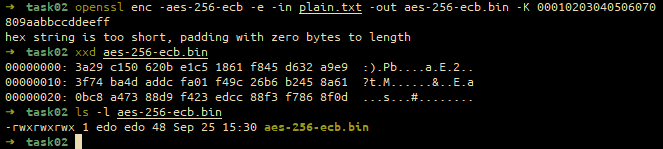
\includegraphics[scale=0.68]{task02_8.png}
    \caption{Cipher type AES-256 with mode ECB.}
\end{figure}

(As expected, it complained about the size of the key being too short, but it
fixed the problem by adding zero bytes without crashing the program)

\begin{figure}[!ht]
    \centering
    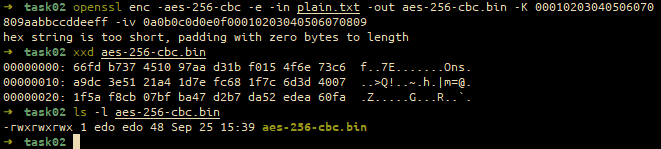
\includegraphics[scale=0.68]{task02_10.png}
    \caption{Cipher type AES-256 with mode CBC.}
\end{figure}

\begin{figure}[!ht]
    \centering
    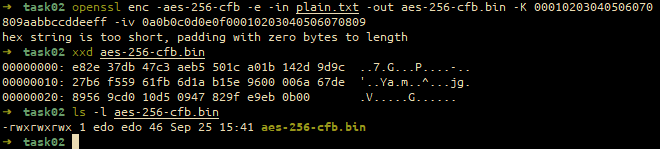
\includegraphics[scale=0.68]{task02_11.png}
    \caption{Cipher type AES-256 with mode CFB.}
\end{figure}

\subsubsection{Observations}
Only in CFB mode that the size of ciphertext is the same as the size of the plaintext.
The two other modes, ECB and CBC, have result ciphertext with size larger than
the plaintext.

The ciphertext generated from different cipher types and modes are different
despite using the same key and initial vector.

\texttt{openssl} automatically patches the wrong the key or initial vector size
by adding zero bytes at the end (to grow the size of them) or ignoring the excess
bytes if the hex string is too long.

\subsection{Task 3: Encryption Mode - ECB vs. CBC}

In this task, I tested encrypting the bitmap image with ECB and CBC mode by
combining them with DES cipher type.

\begin{figure}[!ht]
    \centering
    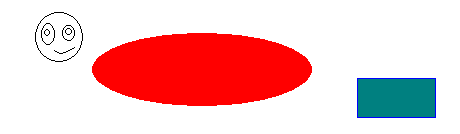
\includegraphics[scale=0.68]{pic_original.png}
    \caption{Original bitmap image.}
\end{figure}

Since the first 54 bytes of bitmap image contains the header information about
the picture, I would like to extract and store it in another file for later use.

\begin{figure}[!ht]
    \centering
    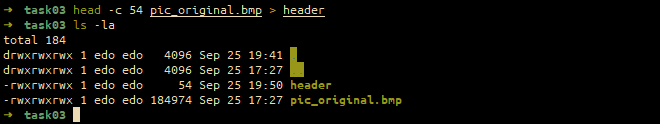
\includegraphics[scale=0.68]{task03_header.png}
    \caption{Extract bitmap header information.}
\end{figure}

The \textbf{key} used in this encryption is \texttt{0001020304050607}.

The \textbf{initial vector} used in this encryption is \texttt{0a0b0c0d0e0f0102}
(the initial vector is not needed in ECB mode).

\begin{itemize}
    \item \textbf{ECB}
        \begin{figure}[!ht]
            \centering
            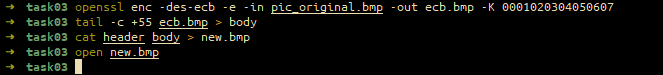
\includegraphics[scale=0.68]{task03_des.png}
            \caption{Encrypt bitmap image with DES cipher type and ECB mode.}
        \end{figure}

        The result bitmap image is shown in Figure 16.

        \begin{figure}[!ht]
            \centering
            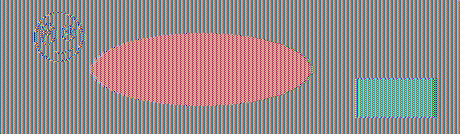
\includegraphics[scale=0.68]{des_ecb.png}
            \caption{Result bitmap image with DES cipher type and ECB mode.}
        \end{figure}

    \item \textbf{CBC}
        \begin{figure}[!ht]
            \centering
            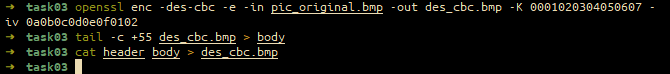
\includegraphics[scale=0.68]{task03_des_2.png}
            \caption{Encrypt bitmap image with DES cipher type and CBC mode.}
        \end{figure}

        The result bitmap image is shown in Figure 18.

        \begin{figure}[!ht]
            \centering
            
\includegraphics[scale=0.68]{des_cbc.png}
            \caption{Result bitmap image with DES cipher type and CBC mode.}
        \end{figure}
\end{itemize}

We can see that the bad guys would definitely get useful information from
bitmap image encrypted with ECB mode since it looks like the original bitmap
image with some noises. The one encrypted with CBC mode does not give us any
useful information from the fact that it looks completely different from the
original.

\subsubsection{Experiment with another picture}

For this experiment, I used the following Illinois Institute of Technology logo
as the original message.

\begin{figure}[!ht]
    \centering
    
\includegraphics[scale=0.68]{IIT.jpg}
    \caption{Original message image.}
\end{figure}

First, I converted the \texttt{jpg} format image to \texttt{bmp} and repeated
the process to get the header information of the original bitmap image and store
it \texttt{header} file.

\begin{figure}[!ht]
    \centering
    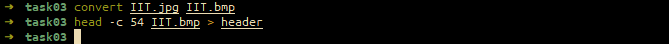
\includegraphics[scale=0.68]{task03_1_header.png}
    \caption{Extract header information from original bitmap image.}
\end{figure}

The \textbf{key} used in this encryption is \texttt{0001020304050607}.

The \textbf{initial vector} used in this encryption is \texttt{0a0b0c0d0e0f0102}
(the initial vector is not needed in ECB mode).

\begin{itemize}
    \item \textbf{ECB}
        \begin{figure}[!ht]
            \centering
            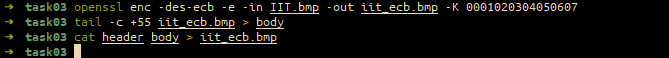
\includegraphics[scale=0.68]{task03_1_des.png}
            \caption{Encrypt bitmap image with DES cipher type and ECB mode.}
        \end{figure}

        The result bitmap image is shown in Figure 22.

        \begin{figure}[!ht]
            \centering
            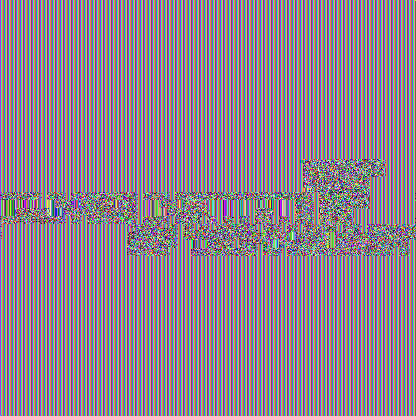
\includegraphics[scale=0.68]{iit_ecb.png}
            \caption{Result bitmap image with DES cipher type and ECB mode.}
        \end{figure}

    \item \textbf{CBC}
        \begin{figure}[!ht]
            \centering
            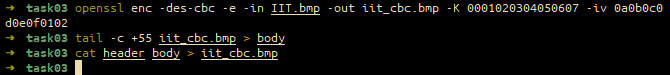
\includegraphics[scale=0.68]{task03_1_des_2.png}
            \caption{Encrypt bitmap image with DES cipher type and CBC mode.}
        \end{figure}

        The result bitmap image is shown in Figure 24.

        \begin{figure}[!ht]
            \centering
            
\includegraphics[scale=0.68]{iit_cbc.png}
            \caption{Result bitmap image with DES cipher type and CBC mode.}
        \end{figure}
\end{itemize}

This time, the information given in encrypted image using ECB mode is harder to
guess since the block data of the unversity name in the image is not exactly
the same so the encrypted data does not look alike. But it still tells us that
the noises in the middle are the important information since it looks much different
than the encrypted white spaces. And we can see the resemblance in the original and
the encrypted image. While the one encrypted with CBC mode looks nothing like
the original, which makes it harder to guess the data in the image.

This is because blocks of data with the same message produce the same
ciphertext using ECB mode. The blocks of message encrypted in
CBC mode are XOR with the initial vector before encryption to create randomnes
in the ciphertext.

\subsection{Task 4: Padding}

\begin{figure}[!ht]
    \centering
    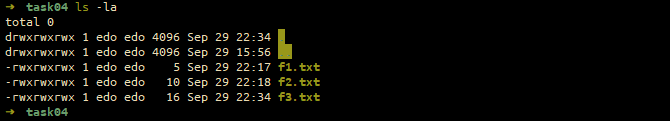
\includegraphics[scale=0.68]{task04_plaintext_files.png}
    \caption{Plaintext files with their size.}
\end{figure}

The content of the plaintext files for 5 bytes, 10 bytes, and 16 bytes are
\texttt{12345} in \texttt{f1.txt}, \texttt{1234567890} in \texttt{f2.txt}, and
\texttt{1234567891011121} in \texttt{f3.txt}.

For the first subtask, I will use \texttt{DES} cipher type with \texttt{ECB},
\texttt{CBC}, \texttt{CFB}, and \texttt{OFB} to encrypt \texttt{f1.txt} file (
the plaintext is \texttt{12345}).

\begin{enumerate}
    \item The \textbf{key} used in this encryption is \texttt{0001020304050607}
        and the \textbf{intital vector} is \texttt{0a0b0c0d0e0f0102}.

        \begin{figure}[!ht]
            \centering
            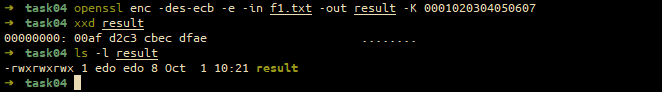
\includegraphics[scale=0.68]{task04_1_ecb.png}
            \caption{Plaintext \texttt{12345} encrypted with DES and ECB.}
        \end{figure}

        \begin{figure}[!ht]
            \centering
            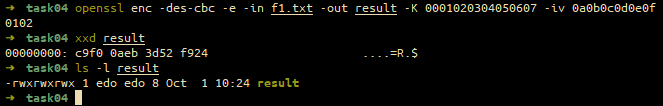
\includegraphics[scale=0.68]{task04_1_cbc.png}
            \caption{Plaintext \texttt{12345} encrypted with DES and CBC.}
        \end{figure}

        \begin{figure}[!ht]
            \centering
            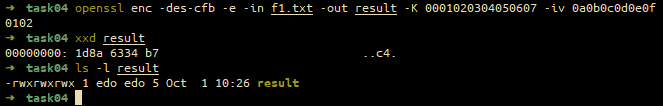
\includegraphics[scale=0.68]{task04_1_cfb.png}
            \caption{Plaintext \texttt{12345} encrypted with DES and CFB.}
        \end{figure}

        \begin{figure}[!ht]
            \centering
            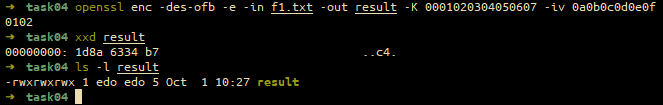
\includegraphics[scale=0.68]{task04_1_ofb.png}
            \caption{Plaintext \texttt{12345} encrypted with DES and OFB.}
        \end{figure}

        The encryption modes that need padding are ECB and CBC (the size of
        plaintext is 5 bytes and the ciphertext is 8 bytes), while CFB and
        OFB does not need padding (the ciphertext size is 8 bytes).

        \begin{figure}[!ht]
            \centering
            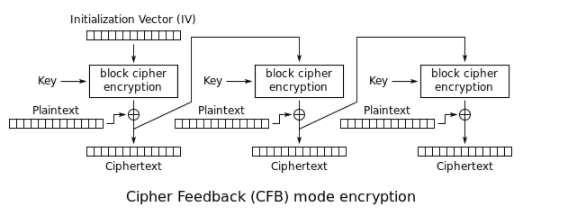
\includegraphics[scale=0.8]{task04_cfb.png}
            \caption{CFB mode encryption.\protect\footnotemark}
        \end{figure}

        \footnotetext{Wikipedia: \url{https://en.wikipedia.org/wiki/Block_cipher_mode_of_operation}}

        \begin{figure}[!ht]
            \centering
            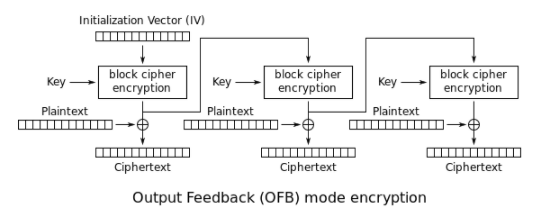
\includegraphics[scale=0.8]{task04_ofb.png}
            \caption{OFB mode encryption.\protect\footnotemark}
        \end{figure}

        \footnotetext{Wikipedia: \url{https://en.wikipedia.org/wiki/Block_cipher_mode_of_operation}}

        This is because in CFB and OFB, the blocks of plaintext are not directly
        used as plaintext for the block cipher encryption, which often requires
        the plaintext to be 128 bits. Instead, the initial vector is used as the
        input for the block cipher encryption and the block of message is only
        used in XOR operation with the result ciphertext of block cipher encryption
        and XOR operation performs on bit by bit of data so it does not require
        any fixed data size.

        On the other hand, ECB and CBC use blocks of plaintext as the input for
        block cipher encryption, which requires the block to be in the size of
        128 bits. So padding is needed for the blocks of plaintext to be in
        the right size to perform the encryption.

    \item The \textbf{key} used in this encryption is \texttt{00010203040506070809aabbccddeeff}
        and the \textbf{initial vector} is \texttt{0a0b0c0d0e0f00010203040506070809}.

        \begin{figure}[!ht]
            \centering
            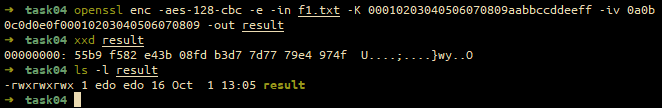
\includegraphics[scale=0.68]{task04_2_e1.png}
            \caption{\texttt{f1.txt} (5 bytes) encrypted with AES-128 and CBC.}
        \end{figure}

        \begin{figure}[!ht]
            \centering
            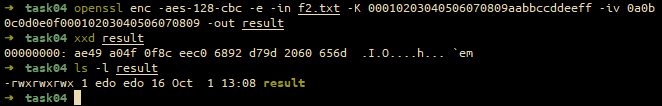
\includegraphics[scale=0.68]{task04_2_e2.png}
            \caption{\texttt{f2.txt} (10 bytes) encrypted with AES-128 and CBC.}
        \end{figure}

        \begin{figure}[!ht]
            \centering
            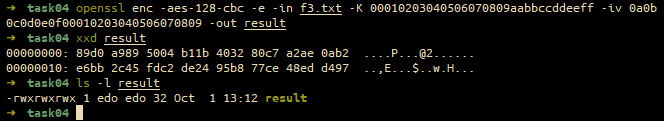
\includegraphics[scale=0.68]{task04_2_e3.png}
            \caption{\texttt{f3.txt} (16 bytes) encrypted with AES-128 and CBC.}
        \end{figure}

        The size of plaintext in \texttt{f1.txt} is 5 bytes and its ciphertext
        is 16 bytes.

        The size of plaintext in \texttt{f2.txt} is 10 bytes and its ciphertext
        is 16 bytes.

        The size of plaintext in \texttt{f3.txt} is 16 bytes and its ciphertext
        is 32 bytes.

        \begin{figure}[!ht]
            \centering
            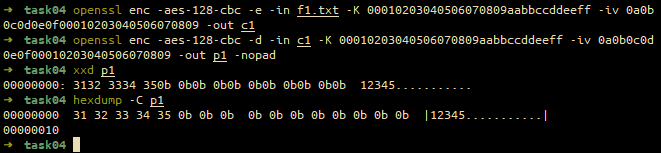
\includegraphics[scale=0.68]{task04_2_d1.png}
            \caption{\texttt{f1.txt} ciphertext decrypted with AES-128 and CBC.}
        \end{figure}

        Hex \texttt{0b} (which is 11 in decimal) is added to the padding during
        encryption of \texttt{f1.txt} because \texttt{f1.txt} block is missing
        11 bytes to be 16 bytes (128 bits).

        \begin{figure}[!ht]
            \centering
            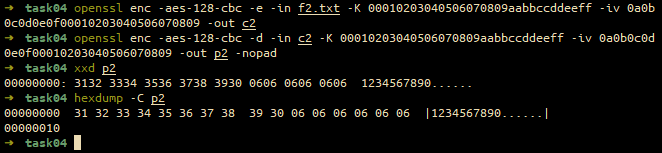
\includegraphics[scale=0.68]{task04_2_d2.png}
            \caption{\texttt{f2.txt} ciphertext decrypted with AES-128 and CBC.}
        \end{figure}

        Hex \texttt{06} (which is 6 in decimal) is added to the padding during
        encryption of \texttt{f2.txt} because \texttt{f2.txt} block is missing
        6 bytes to be 16 bytes (128 bits).

        \begin{figure}[!ht]
            \centering
            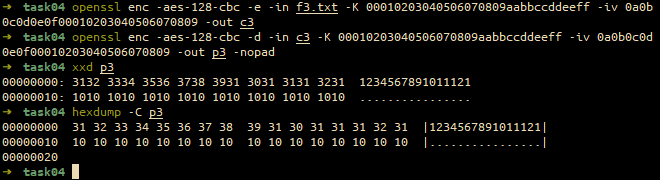
\includegraphics[scale=0.68]{task04_2_d3.png}
            \caption{\texttt{f3.txt} ciphertext decrypted with AES-128 and CBC.}
        \end{figure}

        Hex \texttt{10} (which is 16 in decimal) is added to the padding during
        encryption of \texttt{f3.txt} because \texttt{f3.txt} block is 16 bytes
        which itself can be a block of message. If we keep the plaintext
        without the padding like that, there will not be randomness in ciphertext
        and every plaintext that is like the one in \texttt{f3.txt} will result
        the same ciphertext after encryption. So we have to add another 16 bytes
        (128 bits) to the padding during the encryption.
\end{enumerate}

\subsection{Task 5: Error Propagation - Corrupted Cipher Text}

ECB should be the cipher mode that has the most information recovered by decrypting
the corrupted file, only the block ciphertext with the corrupted byte will not
be fully recovered. This is due to the fact that each block of message is
encrypted seperately and merged together at the end in ECB mode. So the corrupted
block will not be able to affect other blocks.

CBC, CFB, and OFB should have the same amount of data recovered from the corrupted
ciphertext, which is much less than the amount of data recovered from ECB mode,
since in each step, it uses the ciphertext or plaintext of the previous step for
encryption, so all other blocks after that step will be affected as well.

The plaintext used in this task is as follow:

\textbf{
Lorem ipsum dolor sit amet, consectetuer adipiscing elit. Aenean commodo ligula
eget dolor. Aenean massa. Cum sociis natoque penatibus et magnis dis parturient
montes, nascetur ridiculus mus. Donec quam felis, ultricies nec, pellentesque eu,
pretium quis, sem. Nulla consequat massa quis enim. Donec pede justo, fringilla
vel, aliquet nec, vulputate eget, arcu. In enim justo, rhoncus ut, imperdiet a,
venenatis vitae, justo. Nullam dictum felis eu pede mollis pretium. Integer
tincidunt. Cras dapibus. Vivamus elementum semper nisi. Aenean vulputate eleifend
tellus. Aenean leo ligula, porttitor eu, consequat vitae, eleifend ac, enim.
Aliquam lorem ante, dapibus in, viverra quis, feugiat a, tellus. Phasellus viverra
nulla ut metus varius laoreet. Quisque rutrum. Aenean imperdiet. Etiam ultricies
nisi vel augue. Curabitur ullamcorper ultricies nisi. Nam eget dui. Etiam rhoncus.
Maecenas tempus, tellus eget condimentum rhoncus, sem quam semper libero, sit amet
adipiscing sem neque sed ipsumu.
}

In this task, I wrote a Python program to automatically flip a bit (I chose the
least significant bit) in the 55th byte of the ciphertext because I do not have
Bless software.

\begin{python}
import sys

from subprocess import check_output


# corrupt one bit in given position of 55th byte of ciphertext
def corrupt(ciphertext: bytes, position: int) -> bytes:

    # split the ciphertext into list of decimal numbers converted from the bytes
    # of the ciphertext
    ciphertext_bytes = list(ciphertext)

    # get the 55th byte
    target_byte = ciphertext_bytes[54]

    # flip the bit at the given position
    new_byte = target_byte ^ (1 << position)

    # change the 55th byte in the ciphertext to the new byte
    ciphertext_bytes[54] = new_byte

    return bytes(ciphertext_bytes)


if __name__ == "__main__":

    if len(sys.argv) == 2:
        try:
            filename = sys.argv[1]

            # read bytes of ciphertext from given filename
            ciphertext = check_output(['cat', filename])

            # corrupt the first bit of 55th byte in the ciphertext
            corrupted_ciphertext_bytes = corrupt(ciphertext, 0)

            # write the result bytes into a file
            f_corrupt = open(f'corrupted_{filename}', 'wb')
            f_corrupt.write(corrupted_ciphertext_bytes)
            f_corrupt.close()

        except FileNotFoundError:
            print("Cannot open file.")
    else:
        print("Please provide a filename.")
\end{python}

And because I was being lazy, I also wrote a bashscript for encrypting the plaintext,
corrupting the ciphertext, and decrypting the corrupted ciphertext.

\lstset{basicstyle=\footnotesize\ttfamily,
  showstringspaces=false,
  commentstyle=\color{gray},
  keywordstyle=\color{blue},
  frame=single,
  rulecolor=\color{gray}
}

\begin{lstlisting}[language=bash]
#!/bin/bash

openssl enc -aes-128-ecb -e -in plaintext.txt -out ecb.bin \
    -K 00010203040506070809aabbccddeeff
openssl enc -aes-128-cbc -e -in plaintext.txt -out cbc.bin \
    -K 00010203040506070809aabbccddeeff \
    -iv 0a0b0c0d0e0f00010203040506070809
openssl enc -aes-128-cfb -e -in plaintext.txt -out cfb.bin \
    -K 00010203040506070809aabbccddeeff \
    -iv 0a0b0c0d0e0f00010203040506070809
openssl enc -aes-128-ofb -e -in plaintext.txt -out ofb.bin \
    -K 00010203040506070809aabbccddeeff \
    -iv 0a0b0c0d0e0f00010203040506070809

python3 corrupt.py ecb.bin
python3 corrupt.py cbc.bin
python3 corrupt.py cfb.bin
python3 corrupt.py ofb.bin

openssl enc -aes-128-ecb -d -in corrupted_ecb.bin -out p_ecb.bin \
    -K 00010203040506070809aabbccddeeff
openssl enc -aes-128-cbc -d -in corrupted_cbc.bin -out p_cbc.bin \
    -K 00010203040506070809aabbccddeeff \
    -iv 0a0b0c0d0e0f00010203040506070809
openssl enc -aes-128-cfb -d -in corrupted_cfb.bin -out p_cfb.bin \
    -K 00010203040506070809aabbccddeeff \
    -iv 0a0b0c0d0e0f00010203040506070809
openssl enc -aes-128-ofb -d -in corrupted_ofb.bin -out p_ofb.bin \
    -K 00010203040506070809aabbccddeeff \
    -iv 0a0b0c0d0e0f00010203040506070809
\end{lstlisting}

\begin{figure}[!ht]
    \centering
    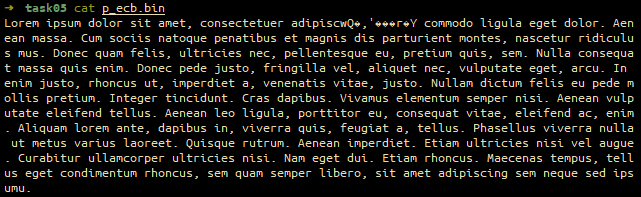
\includegraphics[scale=0.68]{task05_ecb.png}
    \caption{Plaintext decrypted from corrupted ciphertext using AES-128 and ECB.}
\end{figure}

\begin{figure}[!ht]
    \centering
    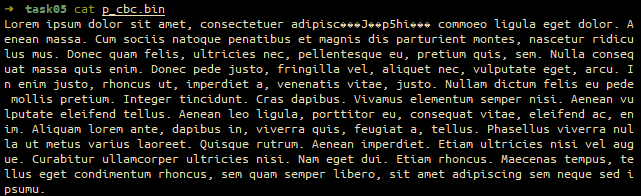
\includegraphics[scale=0.68]{task05_cbc.png}
    \caption{Plaintext decrypted from corrupted ciphertext using AES-128 and CBC.}
\end{figure}

\begin{figure}[!ht]
    \centering
    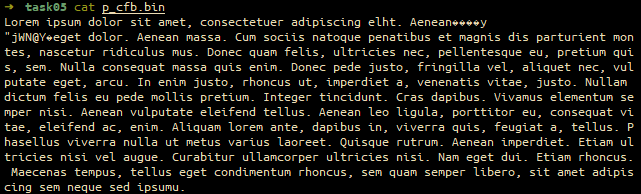
\includegraphics[scale=0.68]{task05_cfb.png}
    \caption{Plaintext decrypted from corrupted ciphertext using AES-128 and CFB.}
\end{figure}

\begin{figure}[!ht]
    \centering
    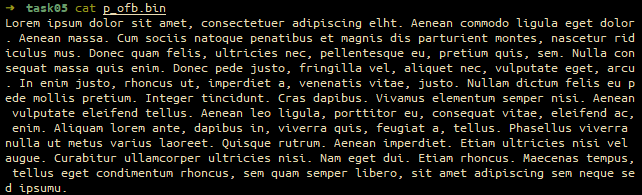
\includegraphics[scale=0.68]{task05_ofb.png}
    \caption{Plaintext decrypted from corrupted ciphertext using AES-128 and OFB.}
\end{figure}

The plaintext of the corrupted ciphertext decrypt using ECB, CBC, CFB, and OFB
mode are shown in Figure 38, 39, 40, and 41.

It seems that my previous answer is wrong, the amount of information can you recover
by decrypting the corrupted file by cipher mode in decreasing order is OFB (only
has one character different from plaintext), CBC (loses two words), ECB (loses
two words), CFB (loses two words and has one character different).

\newpage

\subsection{Task 6: Inital Vector (IV)}

\subsubsection{Task 6.1. Uniqueness of the IV}

The plaintext is \texttt{"This is a secret tool"}.

The \textbf{key} is \texttt{00010203040506070809aabbccddeef}.

The first \textbf{initial vector} is \texttt{0a0b0c0d0e0f00010203040506070809}.

The second \textbf{initial vector} is \texttt{0a0b0c0d0e0f01020304050607080900}.

\begin{figure}[!ht]
    \centering
    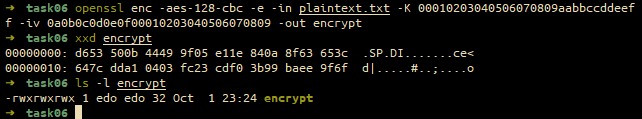
\includegraphics[scale=0.68]{task06_1_1.png}
    \caption{Encrypted plaintext with AES-128 and CBC with first initial vector.}
\end{figure}

\begin{enumerate}
    \item Figure 43 shows the result of encryption using the different IVs.
        \begin{figure}[!ht]
            \centering
            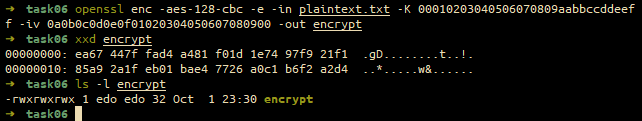
\includegraphics[scale=0.68]{task06_1_2.png}
            \caption{Encrypted plaintext with AES-128 and CBC with different initial vector.}
        \end{figure}
    \item Figure 44 shows the result of encryption using the same IVs.
        \begin{figure}[!ht]
            \centering
            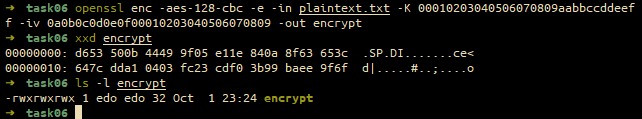
\includegraphics[scale=0.68]{task06_1_1.png}
            \caption{Encrypted plaintext with AES-128 and CBC with same initial vector.}
        \end{figure}
\end{enumerate}

Using the same IVs to decrypt the message results the same ciphertext. Using
different IVs would result different ciphertexts.

Thus, IVs should be different while encrypting the same message to add randomness
to the ciphertext and makes it harder to guess the plaintext based on the ciphertext.

\subsubsection{Task 6.2. Common Mistake: Use the Same IV}

For OFB mode, If the key and IV keep unchanged, known-plaintext attack is feasible.

Output stream can be obtained by XORing plaintext and ciphertext block by block.
Similarly, to get plaintext, I can XOR plaintext and ciphertext. When sharing the
same key and IV for OFB mode, the output streams are identical among encryptions.

We know that \texttt{C1} = \texttt{P1 XOR IV}, then \texttt{IV} = \texttt{P1 XOR C1}.
Thus, \texttt{C2} = \texttt{P2 XOR IV} tells us that \texttt{P2} = \texttt{C2 XOR
IV} = \texttt{C2 XOR P1 XOR C1}.

\begin{python}
from binascii import unhexlify

# initialize p1, c1, c2
p1 = "This is a known message!"
c1 = "a469b1c502c1cab966965e50425438e1bb1b5f9037a4c15913"
c2 = "bf73bcd3509299d566c35b5d450337e1bb175f903fafc15913"

# extract the given p1, c1, c2 to array of bytes
p1 = list(p1.encode('utf-8'))
c1 = list(unhexlify(c1))
c2 = list(unhexlify(c2))

# perform each byte of p1, c1, c2, decode the byte and join it to find p2
p2 = bytes([p1[i] ^ c1[i] ^ c2[i] for i in range(len(p1))]).decode('utf-8')

print(p2)
\end{python}

The result of \texttt{P2} is found to be \texttt{Order: Launch a missle!}.

We can also see that same characters in \texttt{P1} and \texttt{P2} are encrypted
the same. For example, the substring \texttt{e!} at the end of the sentence of \texttt{P1}
and \texttt{P2} is encrypted the be \texttt{c15913}.

\texttt{CFB} would be attacked with the same method above and \texttt{P2} will
be fully revealed.

\subsubsection{Task 6.3. Common Mistake: Use a Predictable IV}

Let the original plaintext sent by Bob is \texttt{P1} and the the next plaintext
is \texttt{P2}.

Construct \texttt{P2} = \texttt{P1 XOR IV XOR IV\_next}.

\begin{python}
from binascii import unhexlify

# guess that the original plaintext is "Yes"
p1 = "Yes"
iv = "31323334353637383930313233343536"
iv_next = "31323334353637383930313233343537"

# convert string to hexadecimal and split them into block of 1 byte
p1 = list(p1.encode('utf-8'))
iv = list(unhexlify(iv))
iv_next = list(unhexlify(iv_next))

# check if plaintext can be split into 128bit-block. If not, add padding to
# the plaintext before encryption
padding = 16 - len(p1) % 16
p1 += [padding] * padding

# calculate p2
p2 = bytes([p1[x] ^ iv[x] ^ iv_next[x] for x in range(len(p1))]).decode("utf-8")
print(p2)
\end{python}

We then check if the ciphertext of \texttt{P2} is the same as the ciphertext of
\texttt{P1}.

\begin{figure}[!ht]
    \centering
    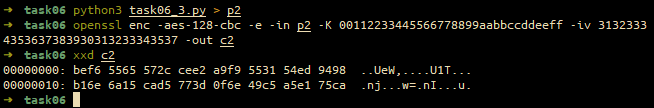
\includegraphics[scale=0.68]{task06_3.png}
    \caption{Check ciphertext generated from \texttt{P2}.}
\end{figure}

We can see that the first few bytes of \texttt{C2} (ciphertext of \texttt{P2})
are the same as the ones in \texttt{C1} (ciphertext of \texttt{P1}). Therefore,
the original message \texttt{P1} is \texttt{"Yes"}.

\subsection{Task 7: Programming using the Crypto Library}

For this task, because there is not any implementation of \texttt{openssl}
encrypt/decrypt library for \texttt{Python}, I used \texttt{pycrypto} \footnote{pycrypto: \url{https://www.dlitz.net/software/pycrypto/api/current/}}
and \texttt{pycryptodome} \footnote{pycryptodome: \url{https://pycryptodome.readthedocs.io/en/latest/src/introduction.html}}
instead.

\begin{python}
from subprocess import check_output

from binascii import unhexlify

from Crypto.Cipher import AES
from Crypto.Util.Padding import pad
from Crypto.Util.Padding import unpad

# read english words from file and store them in an arraylist
f = open("english_word_list.txt")
english_words = f.readlines()
english_words = [x.strip("\n") for x in english_words]
f.close()

# add padding to words so their size is 128 bits
english_words_padding = []

for w in english_words:
    wb = w.encode('utf-8')
    if len(wb)*8 < 128:
        english_words_padding.append(w + "#"*(128//8 - len(wb)))

# to make sure it works right, loop through the list and test if the words are
# 128 bits
for w in english_words_padding:
    if len(w.encode('utf-8'))*8 != 128:
        raise Exception("Key size is too small (less than 128 bits)!!!")

# initialize the plaintext, ciphertext, and initial vector
plaintext = "This is a secret tool"
iv = "010203040506070809000a0b0c0d0e0f"
ciphertext = "ece6753e938f8f903cabbbe12d395bf5f7eae38ad918a2d3e1c3a832476d5c7a"


# in this function, I used openssl to get the key for to compare with the result
# of encryption without using openssl
def enc_openssl(plaintext: str, key: str, iv: str) -> bytes:

    encrypted = check_output(['echo', '-n', plaintext, '|', 'openssl', 'enc',
                              '-aes-128-cbc', '-e', '-K', key, '-iv', iv])

    return encrypted


# encrypt message using aes-128-cbc with pycrypto and pycryptodome library
def enc(plaintext: str, key: str, iv: str) -> bytes:

    key = unhexlify(key)
    iv = unhexlify(iv)

    # initialize the cipher type and mode
    cipher = AES.new(key, AES.MODE_CBC, iv)

    # encrypt the message using the cipher type and mode declared above.
    # also add padding to the plaintext in case the size of blocks of message
    # from plaintext is smaller than 128 bits.
    encrypted = cipher.encrypt(pad(plaintext.encode('utf-8'), AES.block_size))

    return encrypted


# decrypt ciphertext using aes-128-cbc with pycrypto and pycryptodome library
def dec(ciphertext: str, key: str, iv: str) -> bytes:

    ciphertext = unhexlify(ciphertext)
    key = unhexlify(key)
    iv = unhexlify(iv)

    # initialize the cipher type and mode
    decipher = AES.new(key, AES.MODE_CBC, iv)

    # decrypt the ciphertext using the cipher type and mode declared above.
    decrypted = decipher.decrypt(ciphertext)

    # check if the decrypted message has padding. If yes, remove the padding and
    # return the unpadded plaintext. Else, return the decrypted message.
    try:
        decrypted = unpad(decrypted, AES.block_size)
    except Exception:
        pass

    return decrypted


if __name__ == "__main__":

    # bruteforce: go through every possible key and encrypt the plaintext.
    # compare the result with the given ciphertext.
    for k in english_words_padding:
        key = k.encode('utf-8').hex()
        encrypted = enc(plaintext, key, iv)

        if encrypted.hex() == ciphertext:
            print(k)
            print("(ENC) The encryption key is:", k.strip("#"))
            break

    # bruteforce: go through every possible key and decrypt the ciphertext.
    # compare the result with the given plaintext.
    for k in english_words_padding:
        key = k.encode('utf-8').hex()
        decrypted = dec(ciphertext, key, iv)

        if decrypted == plaintext.encode('utf-8'):
            print("(DEC) The encryption key is:", k.strip("#"))
            break
\end{python}

I used two methods to find the encryption key: go through every key to encrypt
the plaintext and compare the result with the given ciphertext, go through
every key to decrypt the ciphertext and compare the result with the given
plaintext. More explanation can be found in the comments in the code.

Both methods result the same key: \texttt{safety\#\#\#\#\#\#\#\#\#\#} with padding
and \texttt{safety} without padding.

\begin{figure}[!ht]
    \centering
    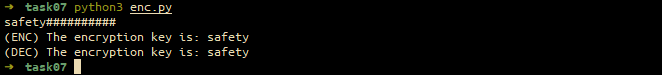
\includegraphics[scale=0.68]{task07.png}
    \caption{Result from running the program above.}
\end{figure}

The result from using \texttt{openssl} is also \texttt{safety\#\#\#\#\#\#\#\#\#\#}
with padding and \texttt{safety} without padding.

Therefore, I can conclude that the encryption key for this cipher is \texttt{safety}.

This method only works if we already know a fixed set of keys that used to
encrypt the message. In real life, the set of possible keys is large and the
key are combination of words and special characters, sometimes the keys do not
have to have meaning, they can be total random. This would make it impossible
to bruteforce AES.

\end{document}
